% Los objetivos específicos de cada uno de los subproyectos participantes, enumerándolos brevemente, con claridad, precisión y de manera realista (acorde con la duración prevista del proyecto).
%
% En los subproyectos con dos investigadores principales, deberá indicarse expresamente de qué objetivos específicos se hará responsable cada uno de ellos.

\subsubsection*{Objectives of the BaTa subproject}
The BaTa subproject will focalize in the development of the laser system and the required technology for an efficient detection of the produced Ba ions resuted from the decay of Xe atoms. The success of this subproject will suppose a great enhancement of the signal-noise ratio of NEXT.

The different objectives of this subproject are:

\begin{itemize}
	\item \textbf{Proof of principle experiment with Ba ions generated by means of an electrical discharge.}
In a first round of experiments we will excite resonantly the S$\leftrightarrow$P transition of Ba$^+$ ions generated by an electrical discharge between two barium electrodes and will collect the fluorescence signal of the P$\rightarrow$D transition (see Fig.\,\ref{fig.levelscheme}). Although this generation method is not ideal because several different species different from Ba ions will be generated, e.g., molecules like BaO or clusters, it does not need a major technological development. It is expected that these initial set of experiments will provide valuable information about the population dynamics in Ba$^+$ ions, and the influence of the different homogenous and inhomogenous broadening mechanisms. It is important to mention that the laser system required for this objective will be provided by the CLPU, and the rest of the material by the ongoing collaboration NEXT-CLPU.
	
\begin{figure}
\centering
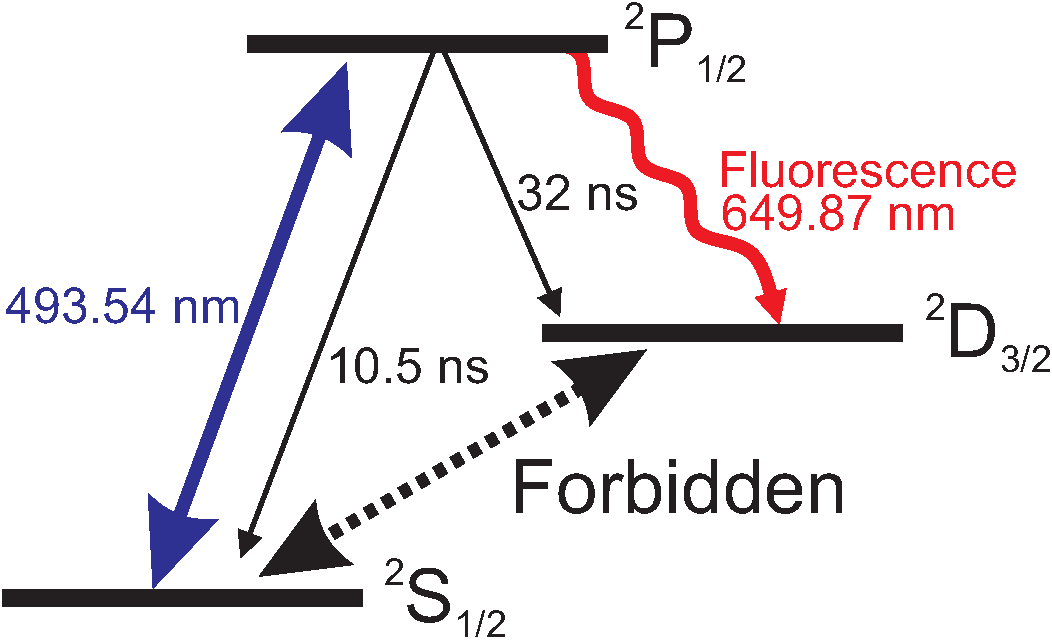
\includegraphics[width=0.5\textwidth]{img/levelscheme.pdf}
\caption{\label{fig.levelscheme} Level scheme for BaTa.} 
\end{figure}
	
	
	\item \textbf{Proof of principle experiment with Ba ions generated by an ion source to be developed.}	
In this objective, in order to get a better approximation of the final conditions of NEXT experiment and with the financial support of a future EXPLORA project, a source of ions will be designed and constructed. This ion source will be based on selective ionization and mass spectrometry techniques, and it will allow a perfect selection of a target specie. Once the source is ready we will repeat the set of experiments of the previous objective but without any parasitic contribution of unwanted compounds. 
	
	
	\item \textbf{Proof of principle experiment with Ba ions generated by means of a developed ion source and with a magneto trap.}	
Once the ion source is in operation, in a following objective, we will develop a magneto trap for Ba$^+$  ions. This trap will allow us to have an excellent degree of control over the experimental conditions and to approach the conditions of NEXT. For instance we will carry out different measurements comparing the collected fluorescence signal as a function of the pressure of the Ba$^+$ ions and the pressure of the surrounding environment. These measurements are mandatory because the population dynamics is really sensitive to pressure, i.e., to collisions. 
	
	
	\item \textbf{Proof of principle experiment with an additional laser for deshelving the D state.}
A possible scenario is that the collisional induced decay between the metastable state D and the ground state S is either not effective or too slow for obtaining an appreciable fluorescence signal. In this situation the population is trapped in the metastable state D  and the fluorescence cycle can not be closed. To avoid this difficulty our approach will be to use a second laser to induce a two photon transition, one photon is forbidden by selection rules, between the states D and S (see Fig.\,\ref{fig.levelscheme2}). This laser must have a wavelength of around 4.1\,$\mu$m which is not easily accesible by commercial laser systems. Our objective is therefore to develop a laser system at this wavelength, and to repeat the experimental matrix defined in previous objectives with two lasers.

\begin{figure}
\centering
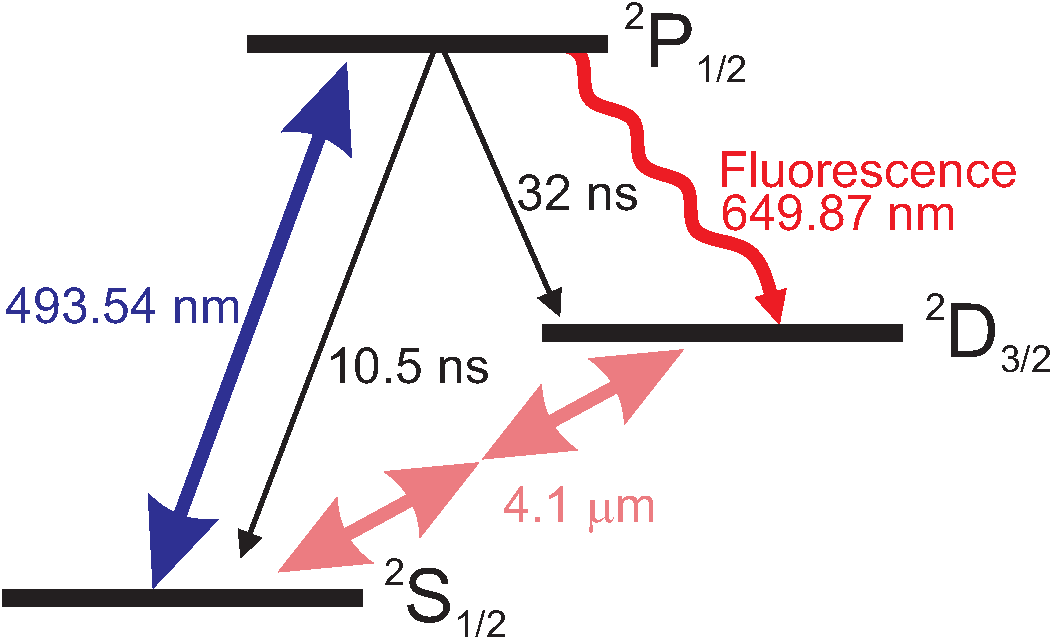
\includegraphics[width=0.5\textwidth]{img/levelscheme2.pdf}
\caption{\label{fig.levelscheme2} Level scheme for BaTa with an infrared deshelving laser.} 
\end{figure}	
	
\end{itemize}

For the successful development of this subproject, CLPU will provide the required human and technological resources. CLPU is the centre of reference in Spain regarding laser technology, and takes active part in several international and national projects. The leader of this subproject will be Alicia V. Carpentier who has a well recognized international trajectory in laser-matter interaction. Moreover, CLPU considers this project of high priority and consequently will offer the collaboration of all the scientific department. This consists of a multidisciplinar team with broad experience in laser technology and development, and laser-matter interaction. 

Furthermore, CLPU will support this project with some of the already operating laser systems in its installation. This is extremely important because such systems usually cost of the order of several hundreds of thousand euros which is totally out of the economical scope of this project. The human resources needed to operate the laser systems will be provided by CLPU as well. We will  also like to mention that the small components needed for the construction of the small prototypes will be afforded by the already established NEXT-CLPU collaboration. For the construction of the ion source, and taking into consideration the specific requirements of this development, we will apply for an \emph{EXPLORA tecnología} in the next call. 

The budget of this subproject will be dedicated to the construction of a red laser of 4.1\,$\mu$m capable of deshelving the D state through a two-photon transition to the ground state. It is important to remark that this specific wavelength is not easily accesible by the commercial laser systems because there are no efficient active media lasing at such wavelength. In fact, nowadays there are big efforts in the laser community devoted to the development of these lasers. This is so because this wavelength is not absorbed by the atmosphere as it lies in what is called the infrared atmospheric window and therefore presents many different technological applications.



